\documentclass{beamer}
\usepackage[utf8]{inputenc}
\usepackage{listings}
\usepackage{svg}

\usetheme{Madrid}
\definecolor{sigaipurple}{rgb}{0.30, 0.16, 0.44}

\useoutertheme{infolines} % Alternatively: miniframes, infolines, split
\useinnertheme{circles}
\usecolortheme[named=sigaipurple]{structure}

\lstset{basicstyle=\footnotesize\ttfamily,breaklines=true}

%------------------------------------------------------------
%This block of code defines the information to appear in the
%Title page
\title[Building Reproducible AI] %optional
{Building Reproducibile AI}

\subtitle{"You wouldn't download a car?"}

\author[SIGAI] % optional
{J.~Setpal} 

\date{October 6, 2022}

\titlegraphic{
\includegraphics[width=5cm]{../shared/logo.png}}

%End of title page configuration block
%------------------------------------------------------------



%------------------------------------------------------------
%The next block of commands puts the table of contents at the 
%beginning of each section and highlights the current section:

\AtBeginSection[]
{
  \begin{frame}
    \frametitle{Table of Contents}
    \tableofcontents[currentsection]
  \end{frame}
}
% ------------------------------------------------------------


\begin{document}

%The next statement creates the title page.
\frame{\titlepage}


%---------------------------------------------------------
% This block of code is for the table of contents after
% the title page
\begin{frame}
\frametitle{Table of Contents}
\tableofcontents
\end{frame}
%---------------------------------------------------------


\section{Why it's Worth Your Time}
%---------------------------------------------------------
%Changing visibility of the text

\begin{frame}{ML as a Science}
	\begin{itemize} 
		\item Foundationally, Machine Learning is a beautiful clusterf*ck. \pause
		\item Proudly. 
		\begin{center}
			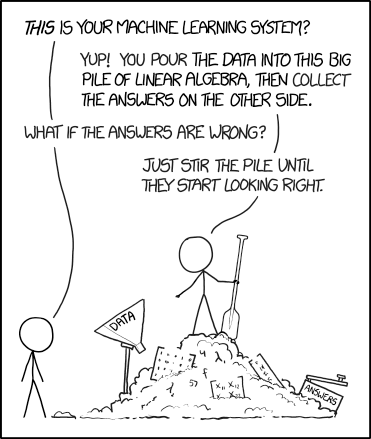
\includegraphics[width=5.4cm]{images/1838}
		\end{center}
	\end{itemize}
\end{frame}

\begin{frame}{ML as a Science}
	\begin{center}
		Imagine having to go debug that.
	\end{center}
\end{frame}

\section{Package Management}

\begin{frame}{Pip}
	\begin{itemize}
		\item Package managers are SAT solvers. 
	\end{itemize}
\end{frame}

\section{Tracking Code}

\begin{frame}{Git}
\end{frame}

\begin{frame}{GitHub}
\end{frame}

\section{Tracking Data}

\begin{frame}{DVC}
\end{frame}

\begin{frame}{MLFlow}
\end{frame}

\begin{frame}{DagsHub}
\end{frame}

\begin{frame}{TensorBoard}
\end{frame}

\section{Project Managment}

\begin{frame}{CookieCutter}
\end{frame}

\begin{frame}{Death to Jupyter Notebooks}
\end{frame}

\begin{frame}{Module-Based Development}
\end{frame}

\begin{frame}{Thank you!}
	\begin{center}
		Have an awesome rest of your day!
	\end{center}
	\begin{center}
		\textbf{Slides:} \texttt{\url{https://cs.purdue.edu/homes/jsetpal/slides/mlops.pdf}}
	\end{center}
\end{frame}

\end{document}
